\chapter{Varianten}

Weitere Varianten des \textit{Apriori}-Algorithmus sind unter anderen \textit{AprioriTID} und \textit{AprioriHybrid}. 
Dabei handelt es sich bei dem Algorithmus \textit{AprioriTID} um eine Erweiterung des \textit{Apriori}-Algorithmus. Während bei dem \textit{AprioriHybrid}-Algorithmus beide Ansätze (\textit{Apriori} und \textit{AprioriTID}) kombiniert werden \parencite[s.][3.2 BFS and Counting Occurences]{VARIANTEN}.

\section{AprioriTID} \label{aprioriTid}
Der AprioriTID stellt eine Erweiterung bzw. Variation des Apriori -Algorithmus da. 
Der Unterschied liegt dabei im zweiten Schritt des Algorithmus (siehe \nameref{alg:apriorigen}). 
Im Gegensatz zum Apriori-Algorithmus wird bei der Erweiterung, die Datenbank $D$ ausschließlich für den ersten Durchlauf verwendet, um den Support zu berechnen. 
Anstelle von $D$ wird für diesen Zweck die Menge $\bar{C}_k$ verwendet. 
Dabei beinhaltet jeder Eintrag den Verweis zur Transaktion ($TID$) sowie eine mögliche häufige Datenmenge ($X_k$). 
Dabei sind in $\bar{C}_k$ nur Einträge vorhanden bei denen die Transaktion\footnote{Über die $TID$ mit $\bar{C}_k$ verbunden} eine Kandidatenmenge ($k-itemset$) enthält. 
Dadurch ist die zugrunde liegende Datenmenge in  $\bar{C}_k$ geringer als die Datenmenge in $D$ (gesamten Transaktionen) bei der Verwendung von Apriori. 


\parencite[s.][2.2 Algorithm AprioriTid]{IBM}

\subsection{Vergleich: Apriori und AprioriTID} \label{subsec:vergleichBasicVsTid}
Auf den ersten Blick suggeriert die Beschreibung des AprioriTID das dieser durch die reduzierten Datenmengen schneller arbeiten sollte.
Diese Annahme ist allerdings nicht immer zutreffend, was in folgenden Test belegt wird \parencite[s.][3.6 Algorithm AprioriHybrid]{IBM}.\\
\\
In den frühen Durchläufen ist die Dauer pro Durchlauf des AprioriTID deutlich langsamer als die Ergebnisse des Apriori. 
Dies ändert sich allerdings im späteren Verlauf (s. Abb.: \ref{fig:aprioriVsAprioriTDI} - \nameref{fig:aprioriVsAprioriTDI}).
Obwohl beide Algorithmen auf die gleiche Art und Weise ihre Kandidaten erzeugen (s. \nameref{aprioriTid} bzw. \nameref{alg:apriorigen}) setzt sich ab dem vierten Durchlauf der AprioriTID durch. 
Dieser Vorsprung basiert darauf, das der AprioriTID nicht die gesamt $D$ (Datenbank) sondern nur die reduzierte Datenmenge $\bar{C}_k$ verwendet \parencite[s.][3.6 Algorithm AprioriHybrid]{IBM}.

\begin{figure}[h]
\centering
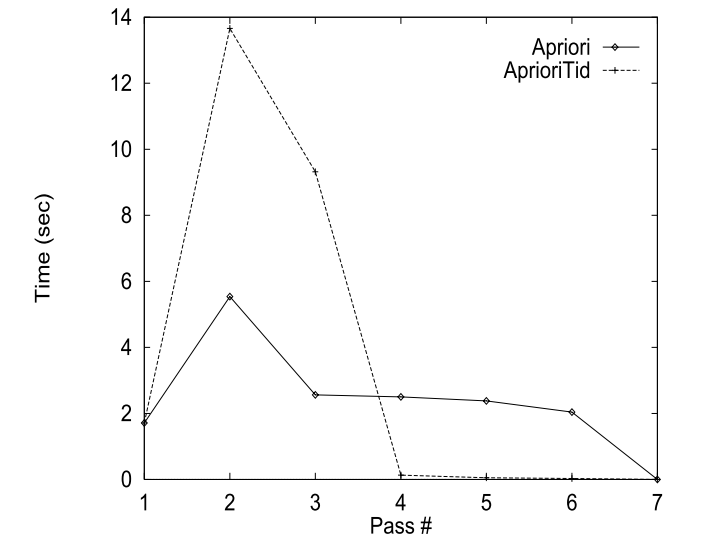
\includegraphics[width=0.7\linewidth]{./images/aprioriVsAprioriTDI}
\caption[Apriori vs AprioriTID]{Vergleich zwischen Apriori und AprioriTID anhand der Dauer pro Durchlauf. Parameter:  Durchschnittliche Größe der Transaktionen = 10, Durchschnittliche Größe der maximalen Kandidatenmenge = 4, Anzahl der Transaktionen = 100.000, minsup = 0.75 \%. \parencite[Quelle:][3.6 Algorithm AprioriHybrid - Figure 6]{IBM}}
\label{fig:aprioriVsAprioriTDI}
\end{figure}


\section{AprioriHybrid}
Das Ziel des AprioriHybrid besteht darin die im letzten Abschnitt (s. \nameref{subsec:vergleichBasicVsTid}) vorgestellten Vorzüge  des Apriori und des AprioriTID zu verbinden (s. Abb.: \ref{fig:hybrid} - \nameref{fig:hybrid}). 
Dieser Hybride Algorithmus verwendet während der Initialisierungsphase den Apriori. 
Dabei wird bei jedem Durchgang geprüft, ob die Größe von $\bar{C}_k \leq$ der Größe des Arbeitsspeichers ist.
Wenn dies der Fall ist wird von Apriori zu AprioriTID gewechselt.
An dieser Stelle ist anzumerken, dass der Wechsel zu AprioriTID mit Kosten verbunden ist. 
Die Entscheidung zum Wechsel wird jeweils am Ende des Durchganges $k$ getroffen. 
Daraufhin wird der Durchgang $k+1$ dafür verwendet, um den AprioriTID zu initialisieren (s. \nameref{aprioriTid}) der schlussendlich erst im Durchgang $k+2$ mit seiner vollen Leistung arbeiten kann \parencite[s.][3.6 Algorithm AprioriHybrid]{IBM}.

\begin{figure}[h]
\centering
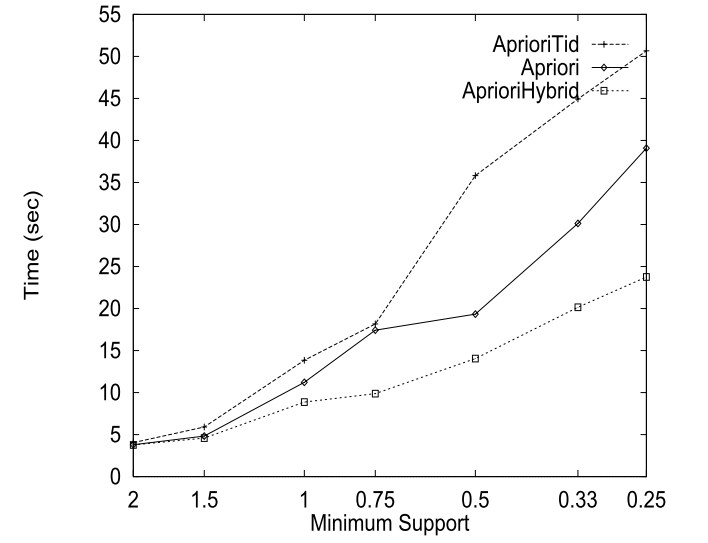
\includegraphics[width=0.7\linewidth]{./images/hybrid}
\caption[Apriori vs AprioriTID vs AprioriHybrid]{Vergleich zwischen Apriori, AprioriTID und AprioriHybrid anhand der Dauer. Parameter: Durchschnittliche Größe der Transaktionen = 10, Durchschnittliche Größe der maximalen Kandidatenmenge = 4, Anzahl der Transaktionen = 100.000 \parencite[Quelle:][3.6 Algorithm AprioriHybrid - Figure 7]{IBM}}
\label{fig:hybrid}
\end{figure}




